\documentclass[../main.tex]{subfiles}

\begin{document}
\subsection{Evoked Responses}
\subsubsection{MEG ERFs}
We first analyzed ERFs time-locked to the onset of the Gabor stimulus. The stimuli were displayed in the right visual field, and we found that the ERFs were strongest in the left posterior electrodes, contralateral to the stimulus presentation (Figure \ref{erfs}). Evoked responses peaked at around 140-200 ms in these posterior electrodes. Although ERFs recorded at an electrode do not necessarily originate from cortical activity directly beneath that electrode, the high activity in the left posterior areas and the lack of activity in the frontal areas and right hemisphere suggest that our MEG signal originated from the left visual area.

\begin{figure}
    \centering
    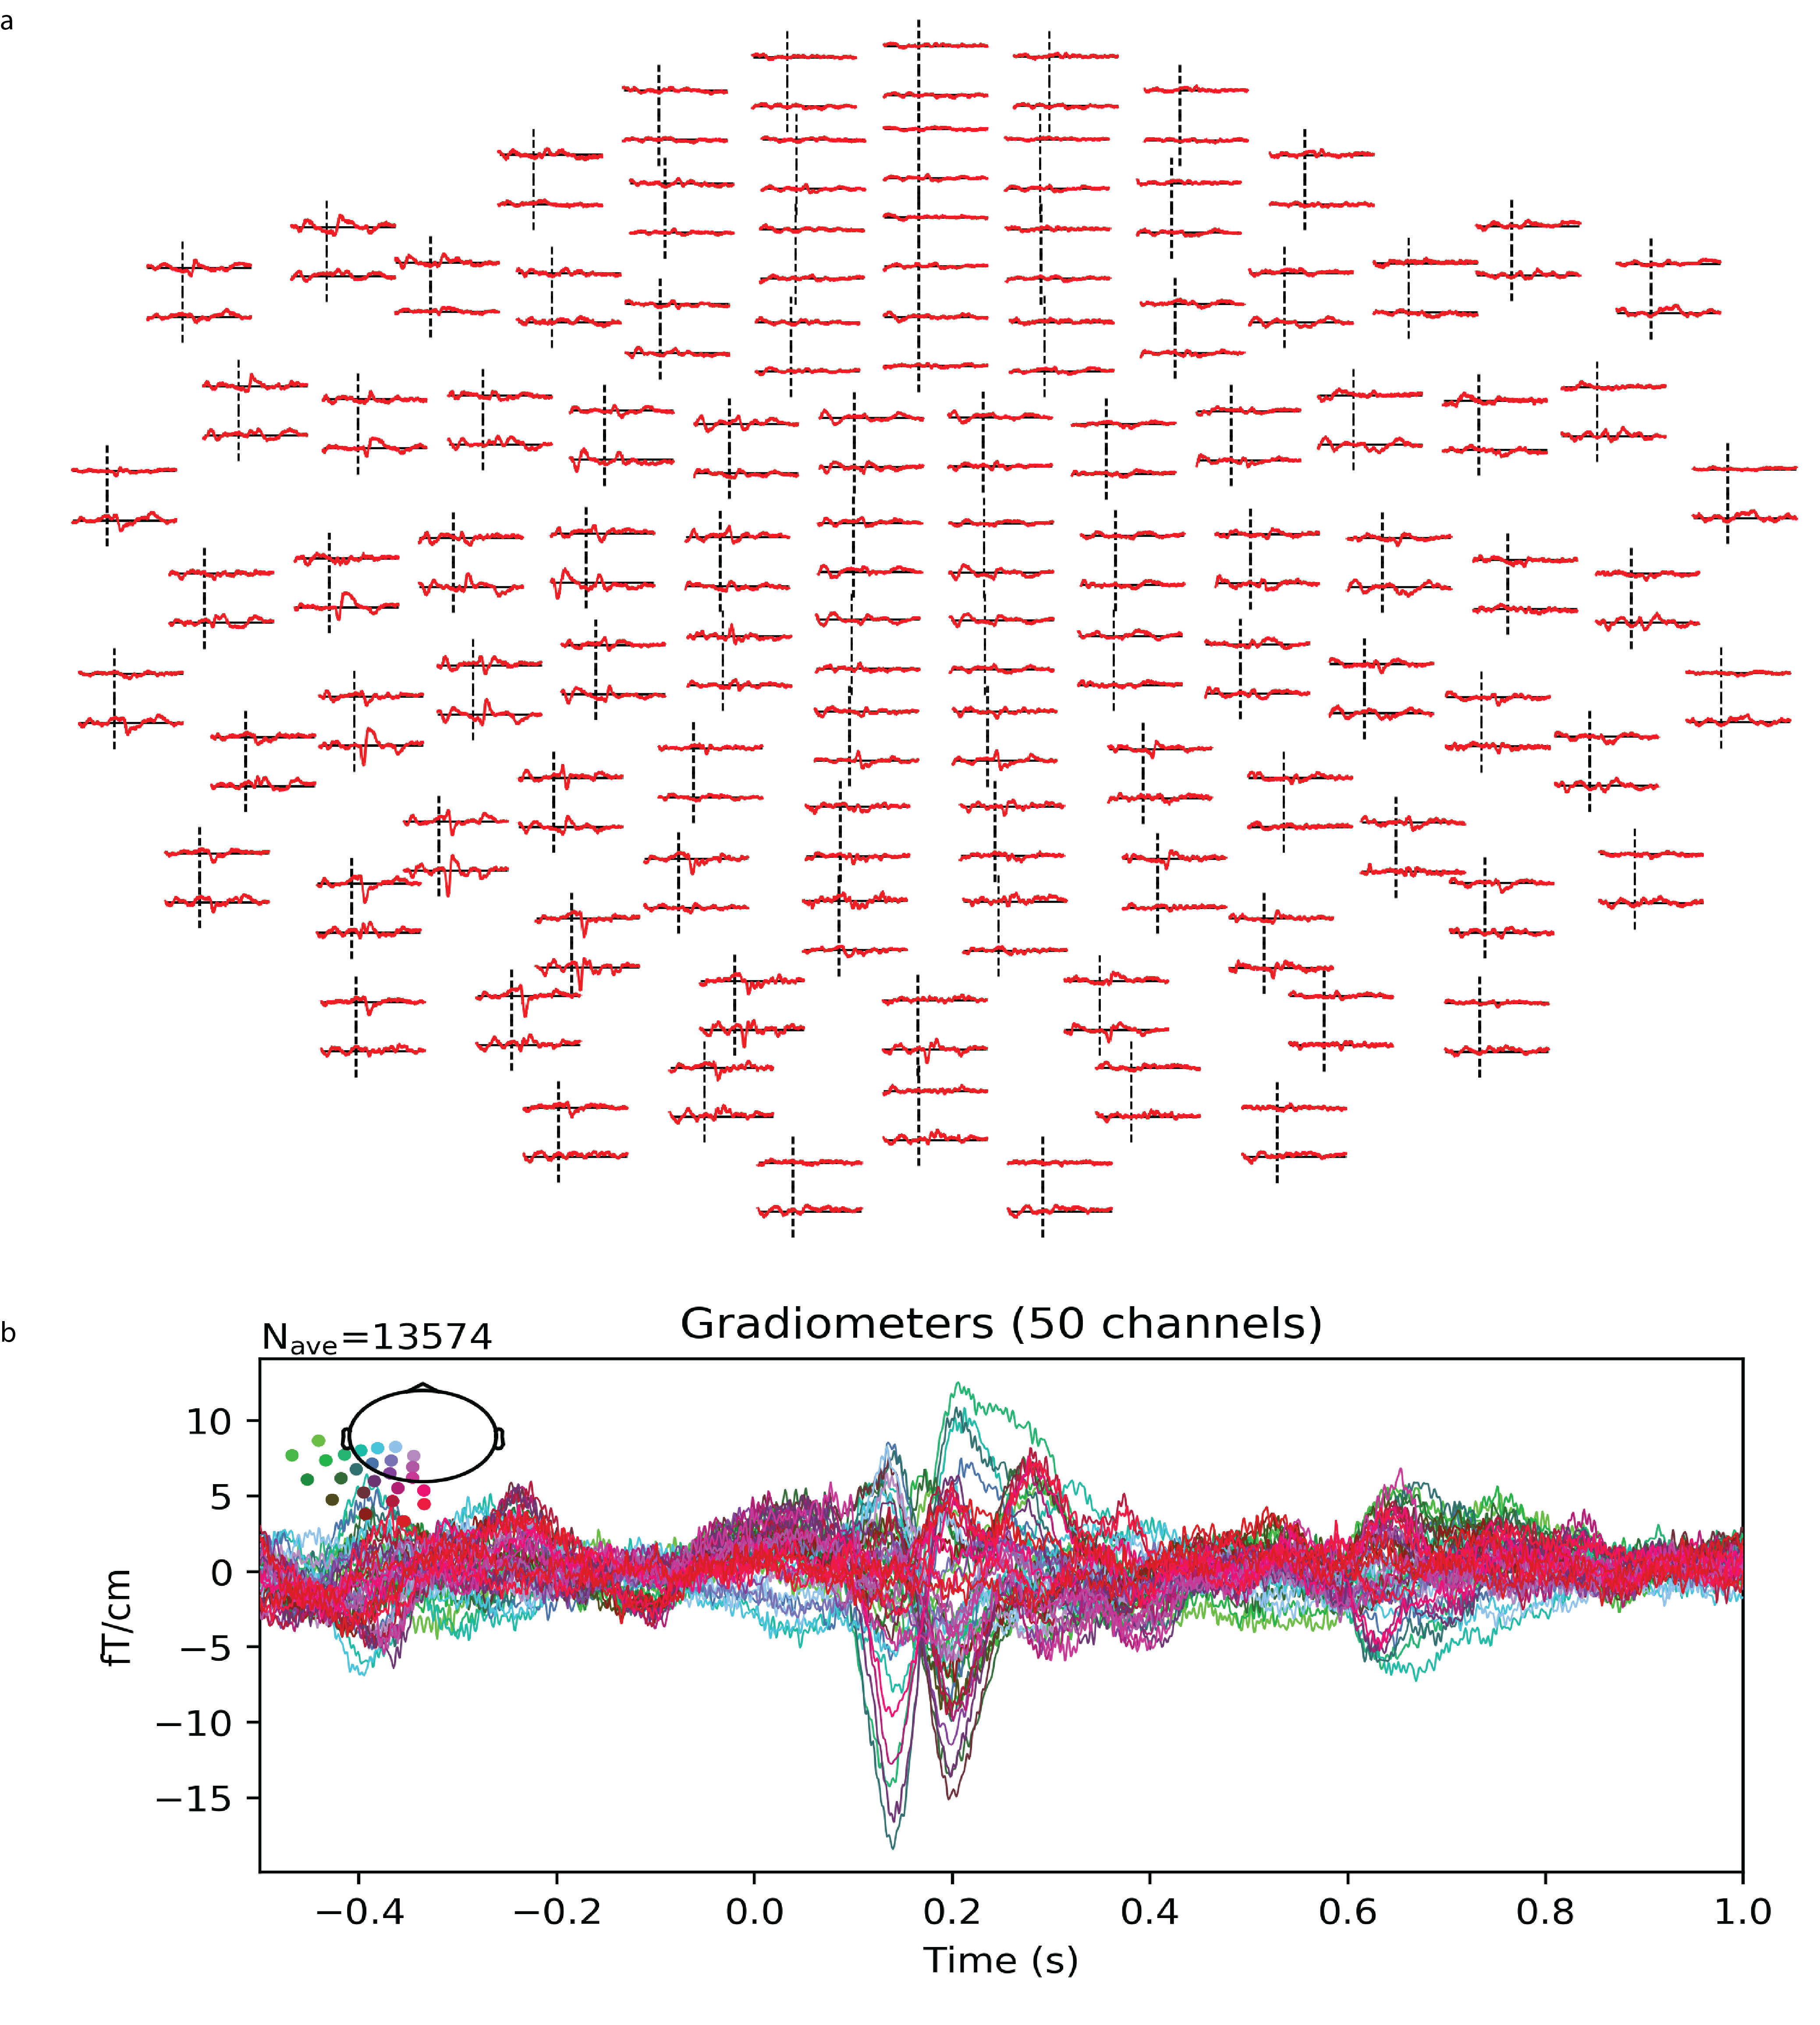
\includegraphics[scale=0.7]{figures/results/erf_results.png}
    \caption{a) Stimulus-onset locked evoked response fields (ERFs) for all electrodes averaged across all subjects. ERFs are strongest in the left posterior electrodes, and ERF peaks begin at 150ms. b) Average ERFs for left occipital and temporal electrodes, from -0.5 to +1.5 seconds.}
    \label{erfs}
\end{figure}


\subsubsection{Source Estimates}
After processing the MEG epochs, we performed a source localization analysis for each subject. In figure \ref{source_max}, we see the averaged source estimate (morphed to the default Freesurfer "fsaverage" subject) for all subjects at the max evoked response time, around 150 ms. Similar to the ERFs, source space activations are localized to left and posterior cortical areas, particularly the visual cortex.

\begin{figure}
    \centering
    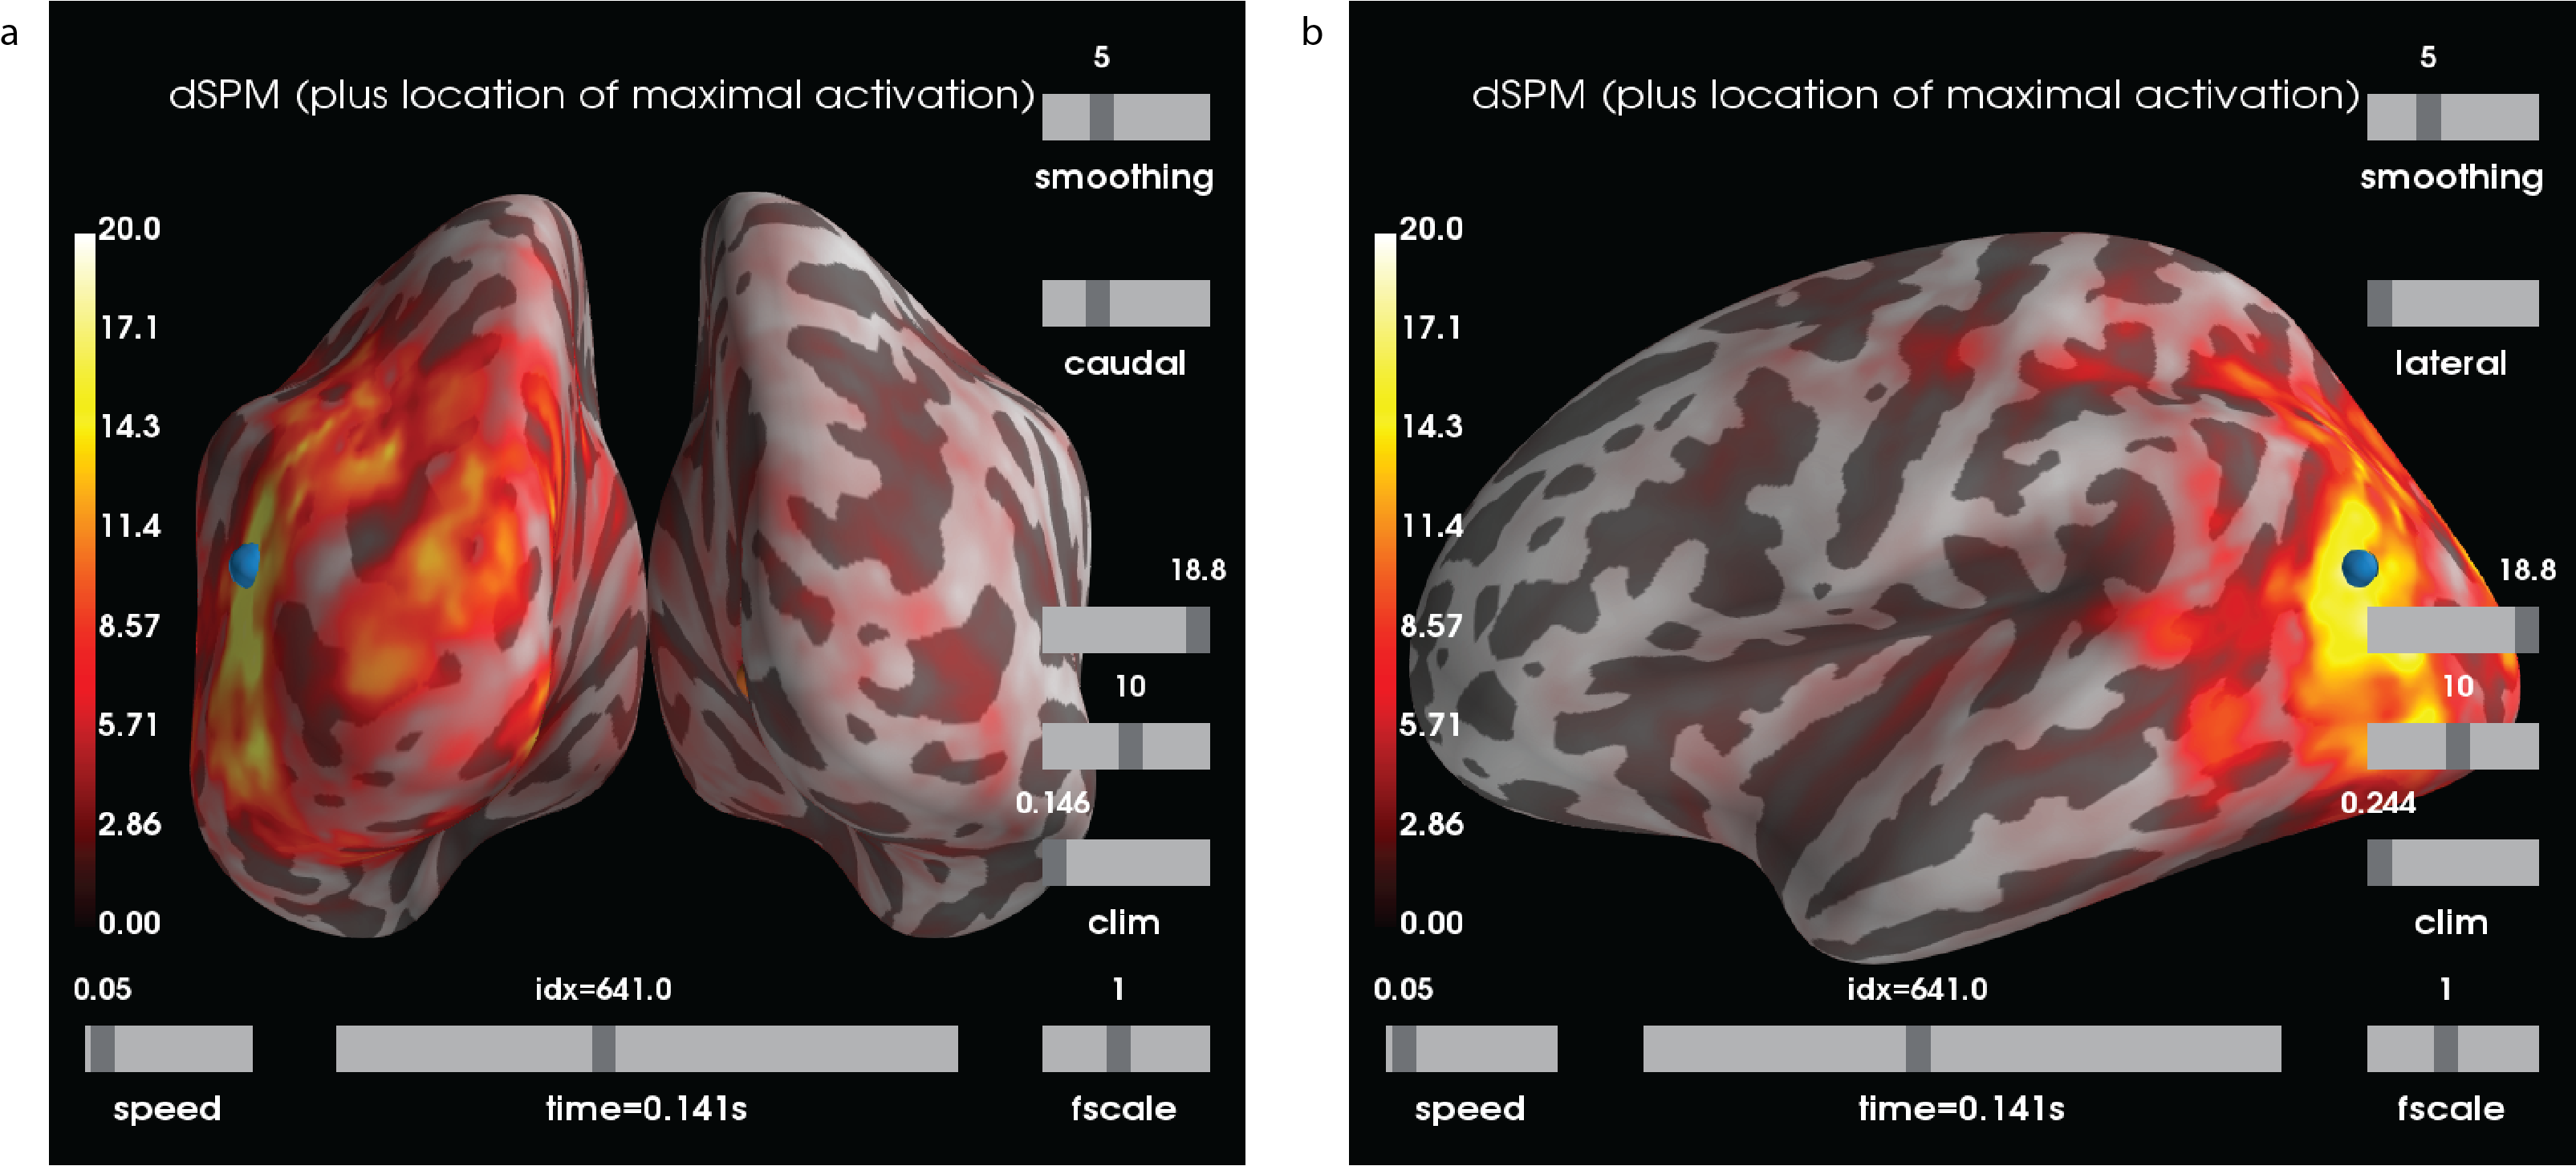
\includegraphics[scale=0.7]{figures/results/source_localiztion_results.png}
    \caption{Peak evoked response for stimulus-locked source estimate data. Activity occurs mainly in the left posterior cortical areas, around the visual cortex. This maximum activity peak occurs at 150ms after stimulus onset.}
    \label{source_max}
\end{figure}


\subsection{Decoding Performance}
\subsubsection{Logistic Regression}
Our first decoding analysis was performed with multi-class logistic regression. Here, we binned Gabor stimuli into 9 groups (i.e. 9 ranges of orientations). We then performed a 5-fold cross-validation on each subject to compute accuracies over 16 time steps from 0 to 375ms milliseconds. We also computed the mean accuracy over all 16 time steps. Each cross-validation was performed 10 times with shuffled data to generate decoding results. One hundred permutation tests were run with permuted data labels to generate permutation results. Figure \ref{logistic_sensor_accuracy} shows the logistic regression accuracy computed at each time step. Here, only one time step has accuracy significantly above the permutation accuracy, at 175 ms after stimulus onset. From 225 to 325 ms, we observed a peaking structure where accuracy increases over each step, but none of these time steps were individually significant. The mean accuracy over all time steps is significant, but with very low accuracy (Figure \ref{logistic_sensor_accuracy}. Variance was very low, as mean accuracies were averaged across all 18 subjects before permutation test comparison. These results suggest that the logistic regression is able to decode orientation, but no significant decoding structure is revealed between time steps. 

We also performed logistic regression decoding with our source localized data. We did not find any significant time steps, nor did we find the mean accuracy to be significant (Figure \ref{logistic_source_accuracy}). This might suggest that the source estimation process introduced noise to the decoding process that reduced decoding accuracy.


\begin{figure}
    \centering
    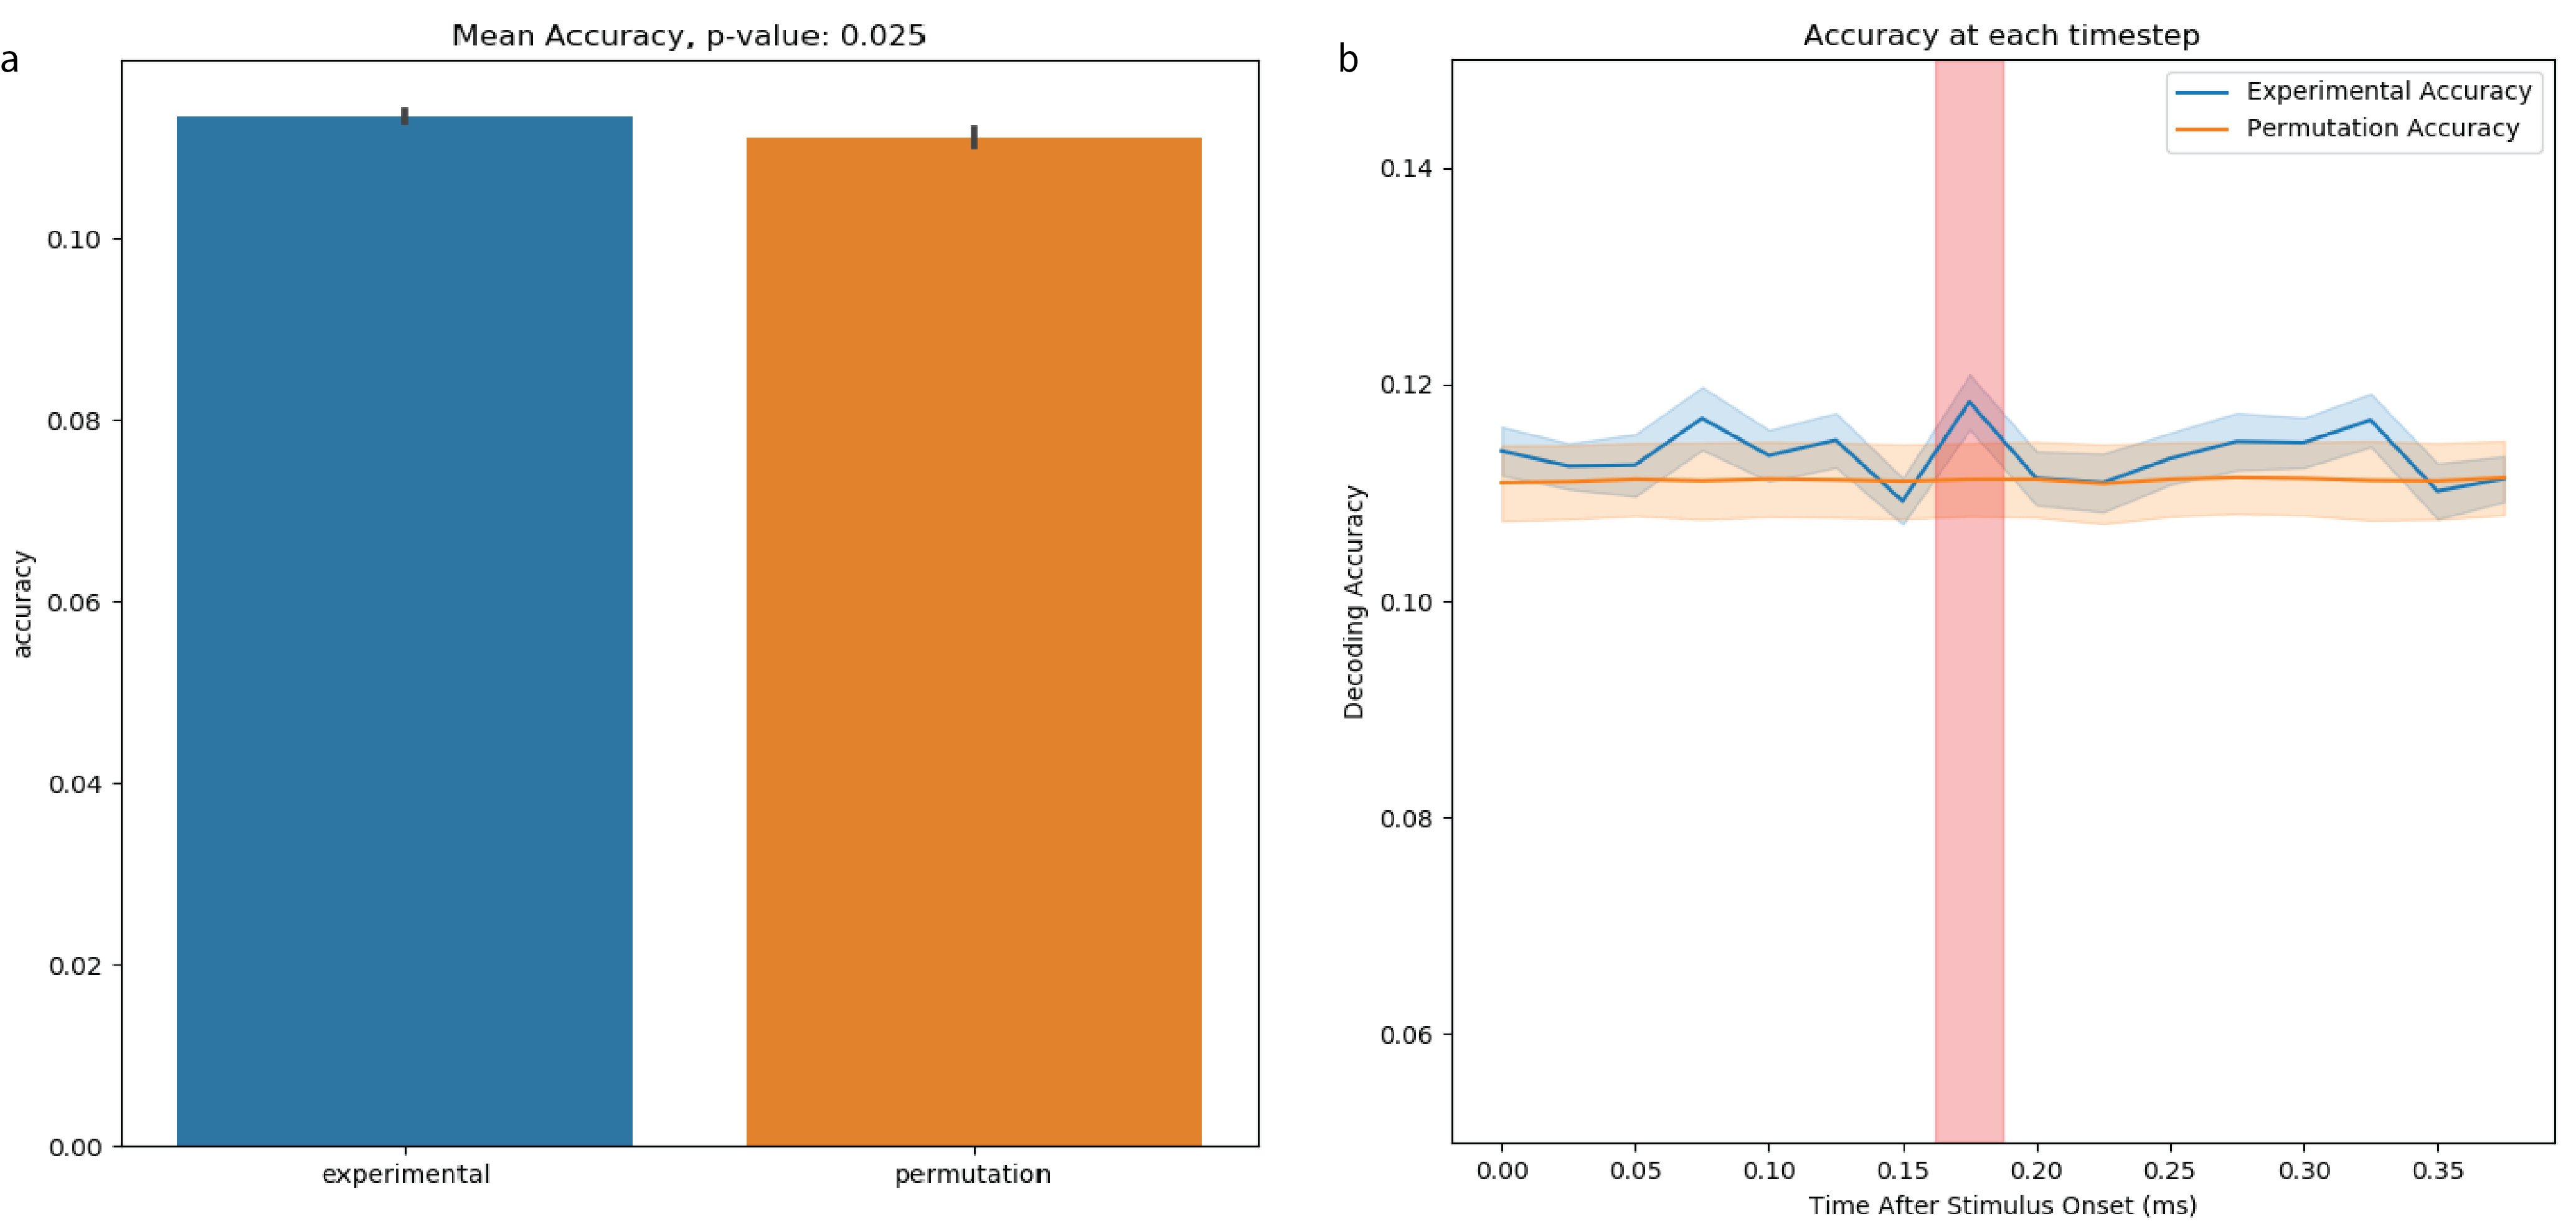
\includegraphics[scale=0.7]{figures/results/logistic_sensor_accuracy.png}
    \caption{a) 5-fold cross-validation accuracy computed at 16 time steps, with standard deviation bars. Accuracies are averaged across 18 subjects. The red highlighted section at 175ms denotes a time step with accuracy significantly above the permutation test decoding accuracy. b) Mean accuracy over all time steps. The experimental model achieves modest accuracy gains over the mean permutation accuracy. Bars indicate standard deviation of accuracy.}
    \label{logistic_sensor_accuracy}
\end{figure}


\begin{figure}
    \centering
    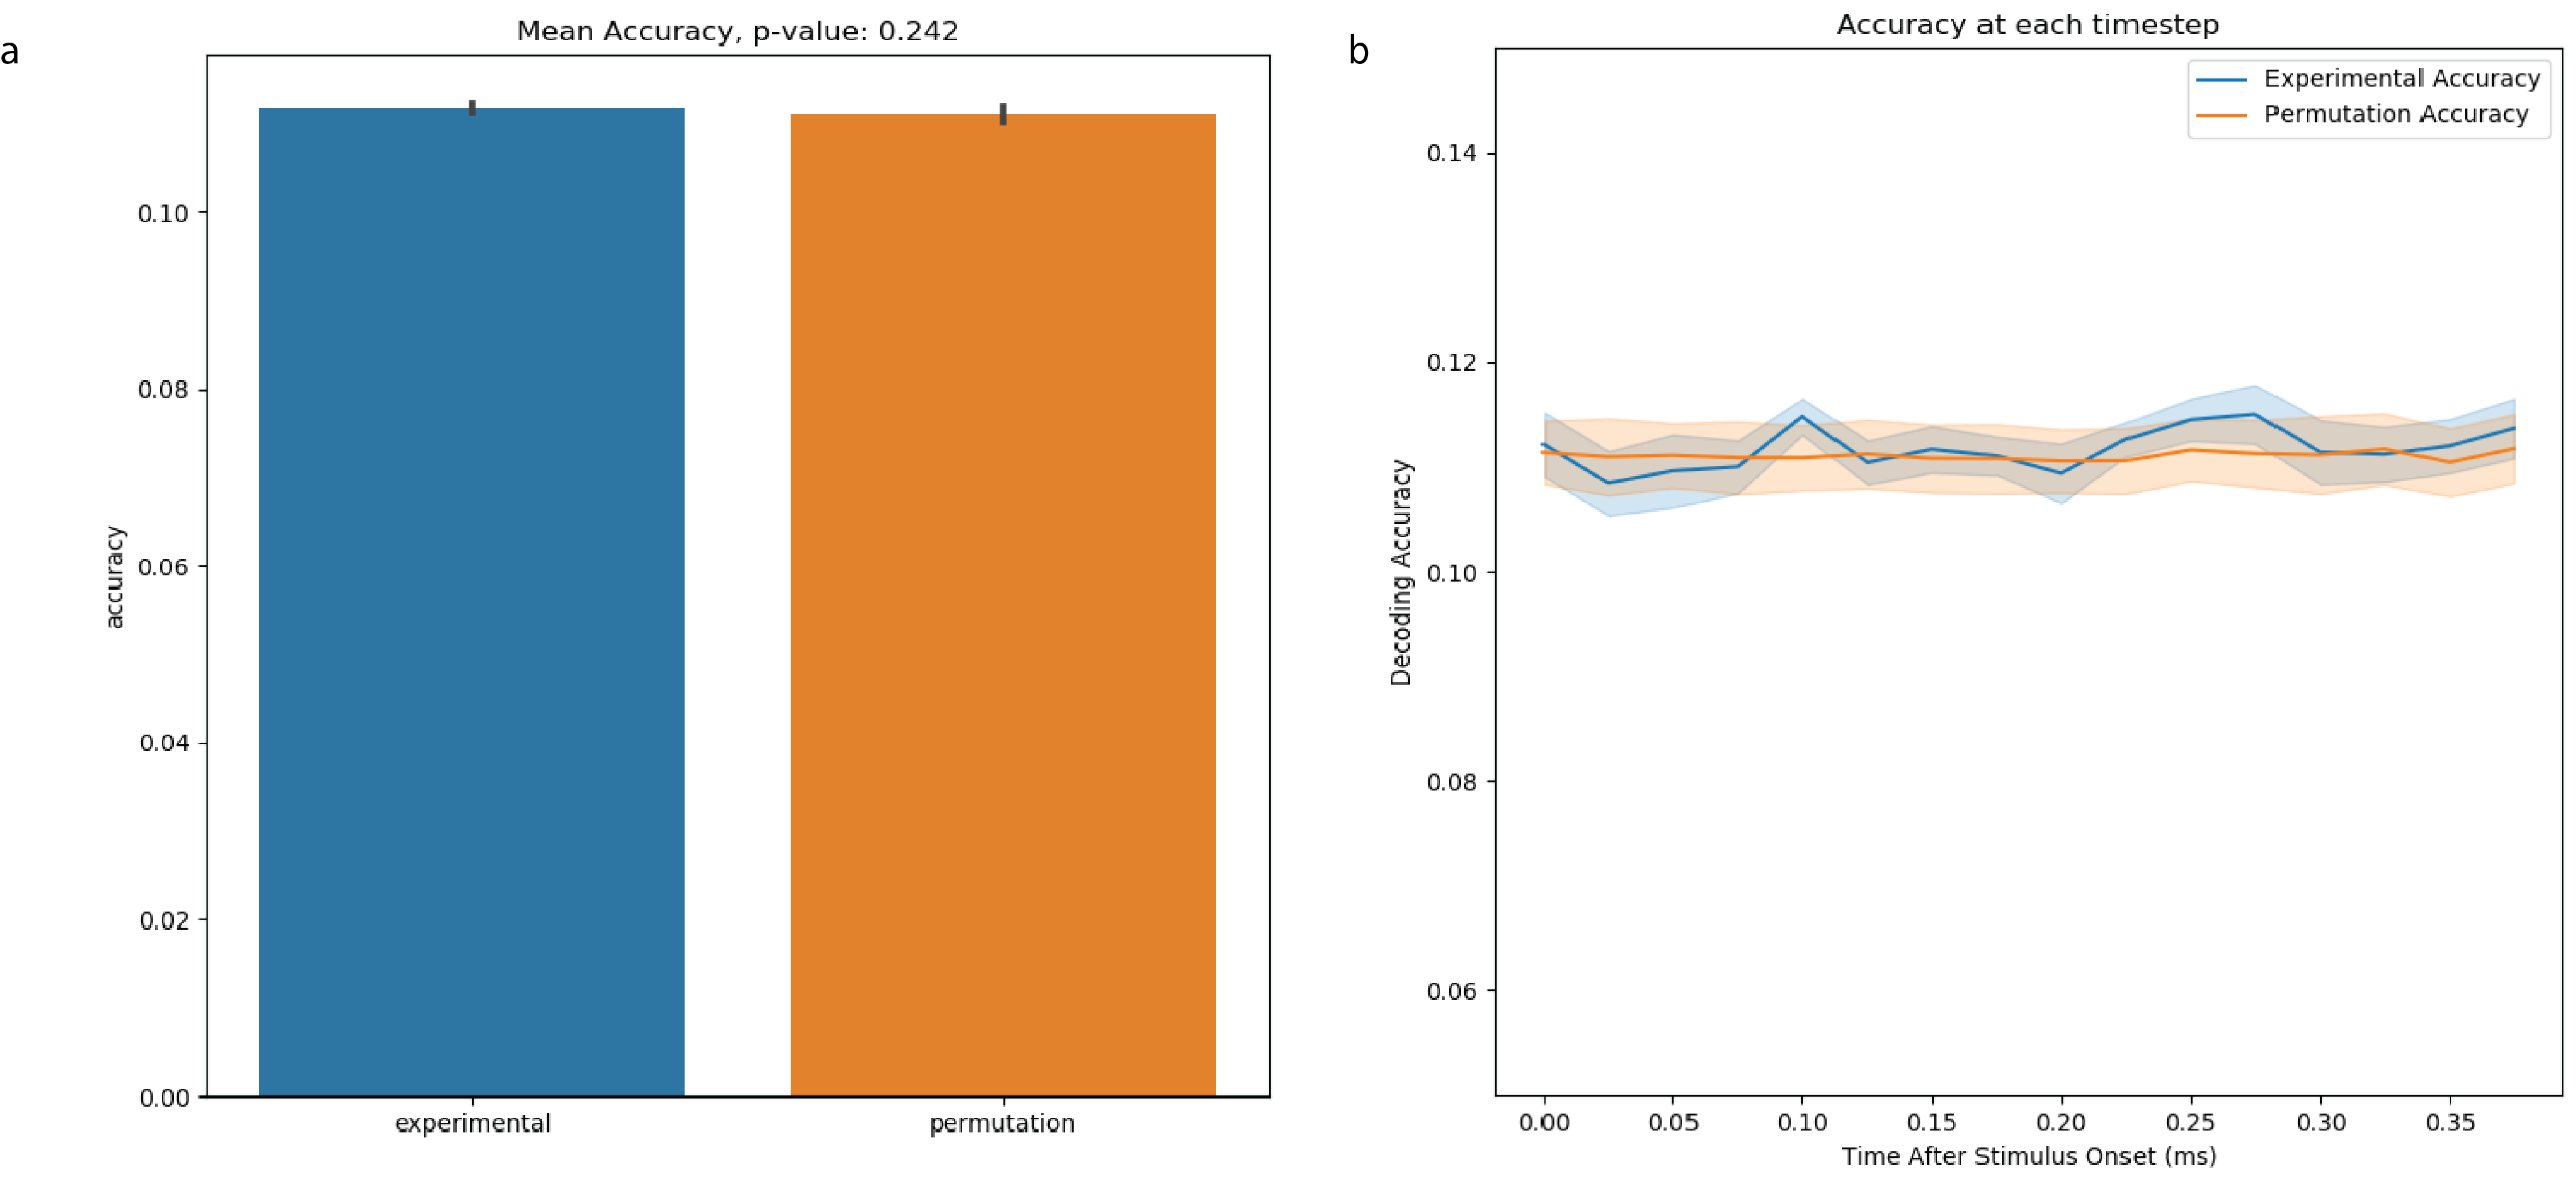
\includegraphics[scale=0.7]{figures/results/logistic_source_accuracy.png}
    \caption{a) Mean accuracy across 16 time steps for 18 subjects using the logistic regression model with source space inputs, compared to permutation test accuracy at 16 time steps. No time steps were significant. b) Mean accuracy over all time steps for the logistic regression model with source space inputs, compared to a permutation test accuracy.}
    \label{logistic_source_accuracy}
\end{figure}

\subsubsection{Support Vector Machine (SVM)}
Similar results were achieved using the same decoding process with an SVM. SVMs are the most commonly used model in multi-variate pattern analysis, or decoding, but we didn't observe any performance increases over the logistic regression model here. In Figure \ref{svm_sensor_accuracy}, there were no individual time points with significant decoding accuracy. Further, while the decoding accuracy was generally above the permutation accuracy at each time step, it also remained within the standard deviation of the permutation time steps. We found a similar upward trend in decoding accuracy beginning around 225 ms as we found in the logistic regression model, but it was again not significant, based on decoding accuracy. Similar to the logistic regression, there was a small, but significant, increase in decoding accuracy in the mean accuracy (p $<$ 0.05, permutation test; Figure \ref{svm_sensor_accuracy}). The variance for mean accuracy was again very low, as the mean accuracy was averaged across 18 subjects before the permutation test.

\begin{figure}
    \centering
    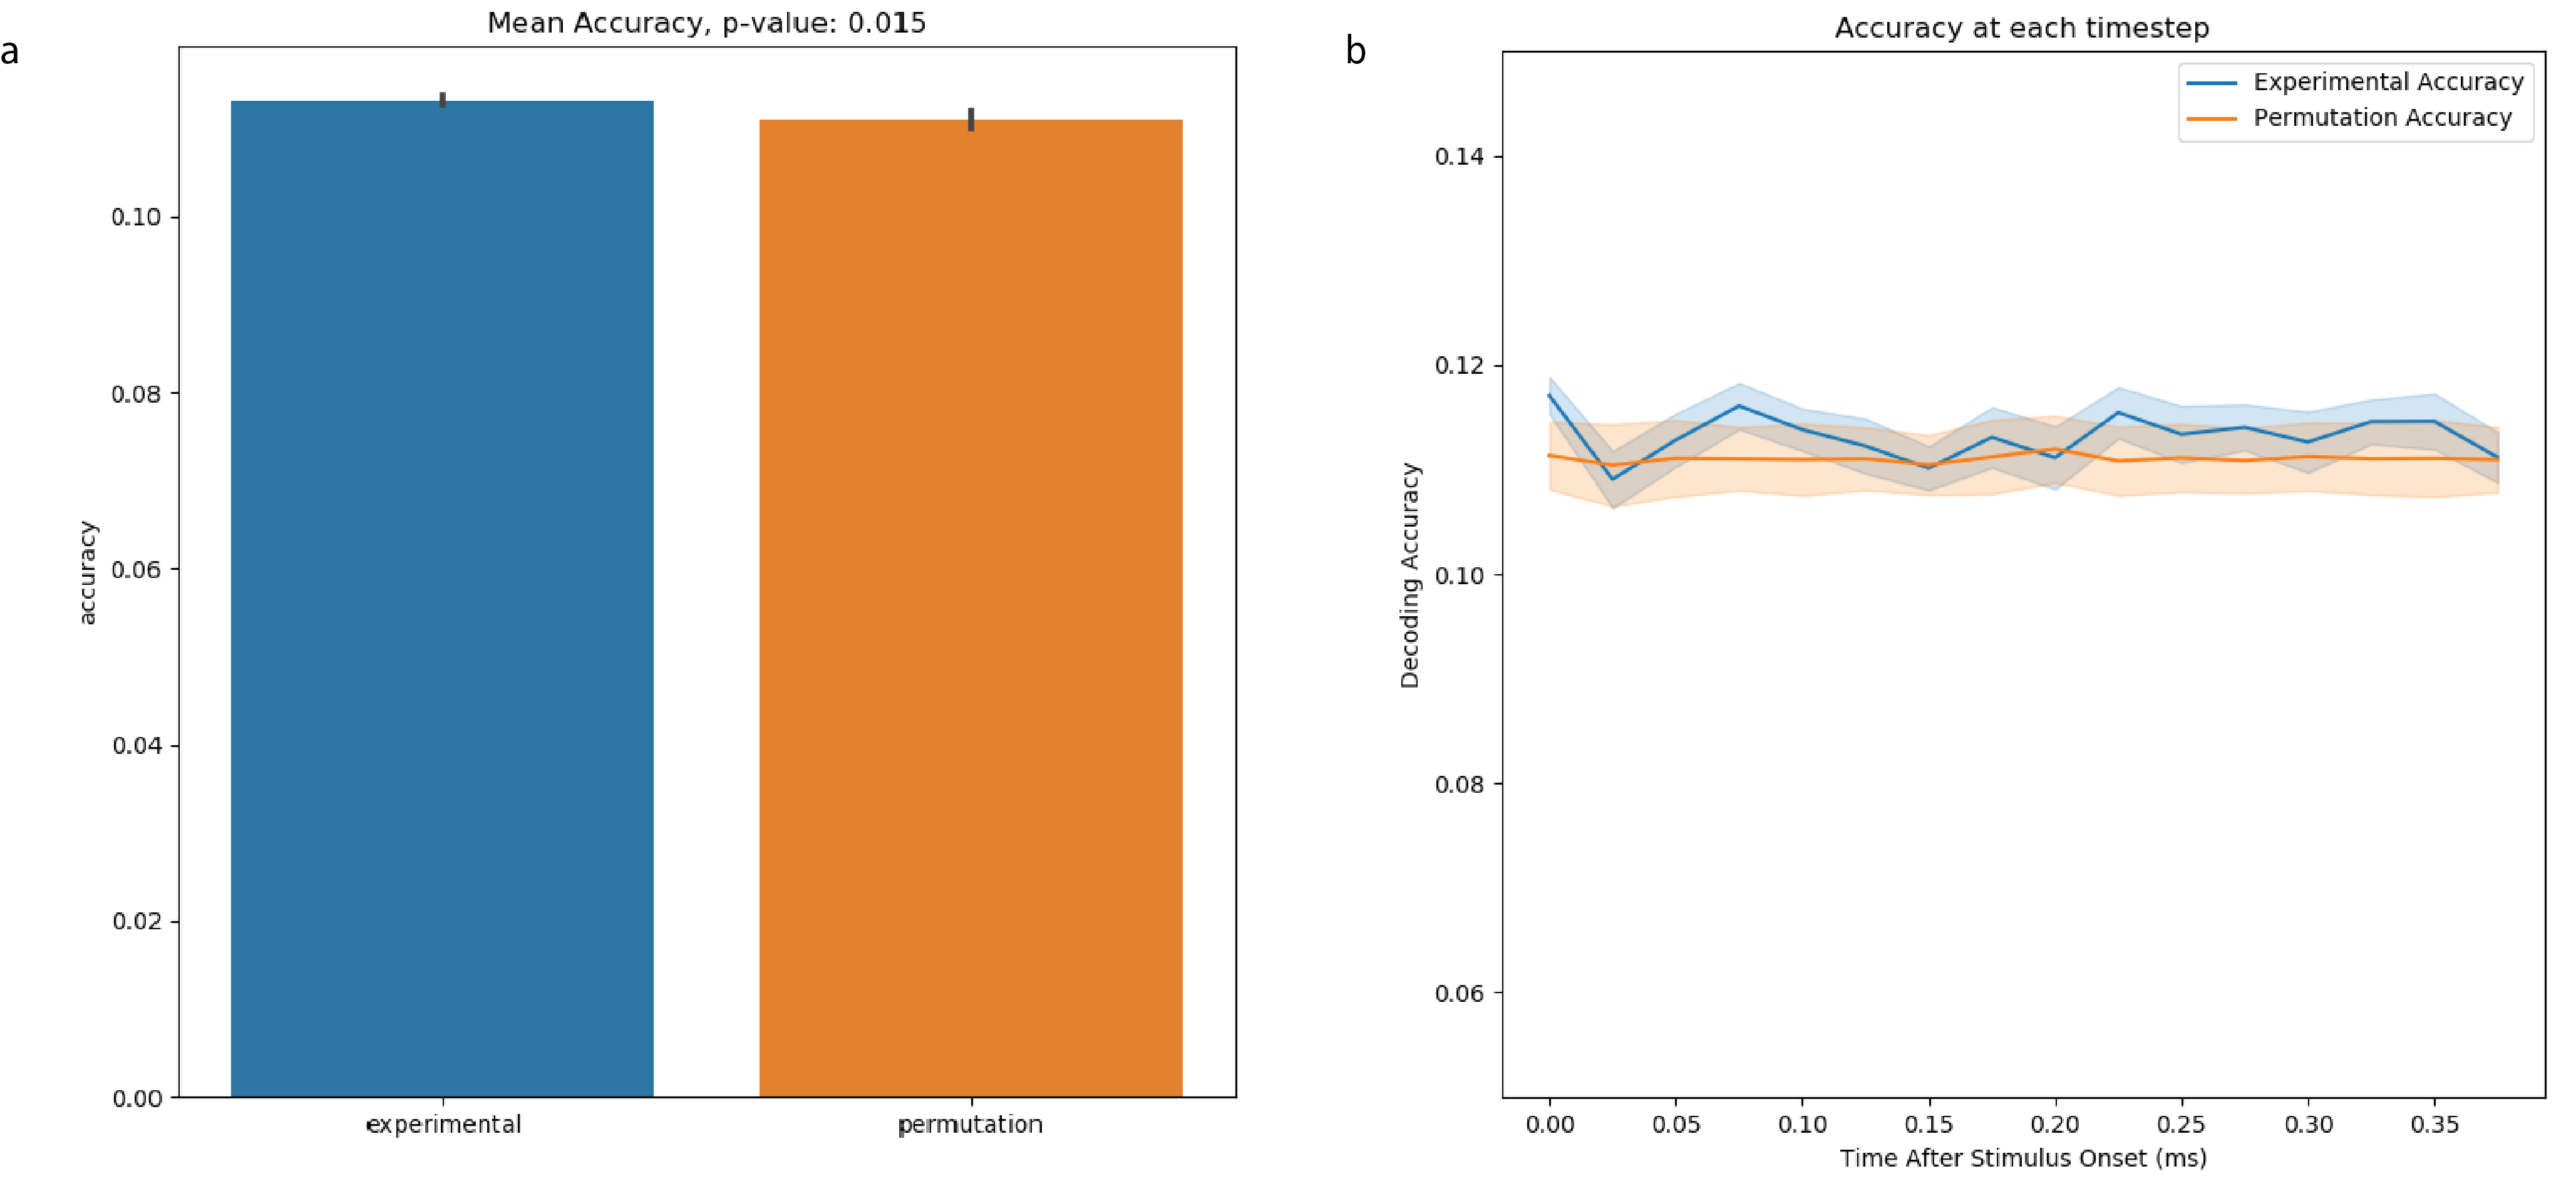
\includegraphics[scale=0.7]{figures/results/svm_sensor_accuracy.png}
    \caption{a) Accuracy at 16 time steps for a support vector machine.  Bars around the line plots indicate standard deviation. No significant accuracies are achieved at any time step. b) Mean accuracy over 16 points for a support vector machine compared to a permutation test. Black bars indicate decoding accuracy standard deviation.}
    \label{svm_sensor_accuracy}
\end{figure}

\subsubsection{Inverted Encoding Model}
We finally looked at the inverted encoding model (IEM) for decoding orientation, and achieved much better results in comparison to the more traditional models. Rather than generating a prediction, the IEM predicts a channel response for each of the orientation channels. This channel response is a prediction of how much a particular orientation is associated with a set of MEG data. In Figure \ref{iem_results}, we first looked at the mean channel response of our experimental IEM in comparison to a permutation test. The mean channel response, centered at 90 degrees for visualization, had a significant bell-curve structure centered at 90 degrees, while the permutation channel response was flat. This indicates that the IEM successfully predicted the highest channel response at the displayed orientation, and that the channel response decreased as a function of distance from the stimulus orientation. This suggests that similar orientations have a similar encoding. These results are in line with findings from other IEM decoding papers, particularly \cite{GARCIA2013515}. However, we reproduced these results with a wider variety of possible orientations and smaller, peripheral Gabor targets. When we looked at the channel response at each time step, we found that the channel response was mostly flat until 175 ms, at which point it increased until it peaked at 225ms, and then decreased again until 375ms. This indicates that channel responses increased after evoked responses, which we found to peak from 150-175ms in the left posterior electrodes.

We then examined the decoding accuracy achieved by the IEM, using the orientation corresponding to the maximum channel response as the orientation prediction for an epoch. We first ran this decoding at each time step, as seen in Figure \ref{iem_results}. Here, we achieved significant decoding accuracy at 3 different time steps, and the decoding accuracy was generally higher than decoding accuracy for the previous models. The accuracy started to increase much earlier, at 125ms, and a sustained peak was observed from 225-350ms. We next computed the accuracy achieved by the mean channel response. Note that unlike previous decoding models, where we computed a mean accuracy by averaging the accuracies achieved over multiple time steps, here we computed the mean channel response and then computed the accuracy of the mean channel response as the percentage of trials where the orientation for the maximum channel response matched the orientation of the stimulus. In Figure \ref{iem_results}, the mean channel response achieved an accuracy significantly above the permutation test. This indicates that the IEM is incredibly successful at decoding orientation from MEG, and decoding accuracy increases following evoked responses in MEG, revealing a significant decoding structure as a function of time.

\begin{figure}
    \centering
    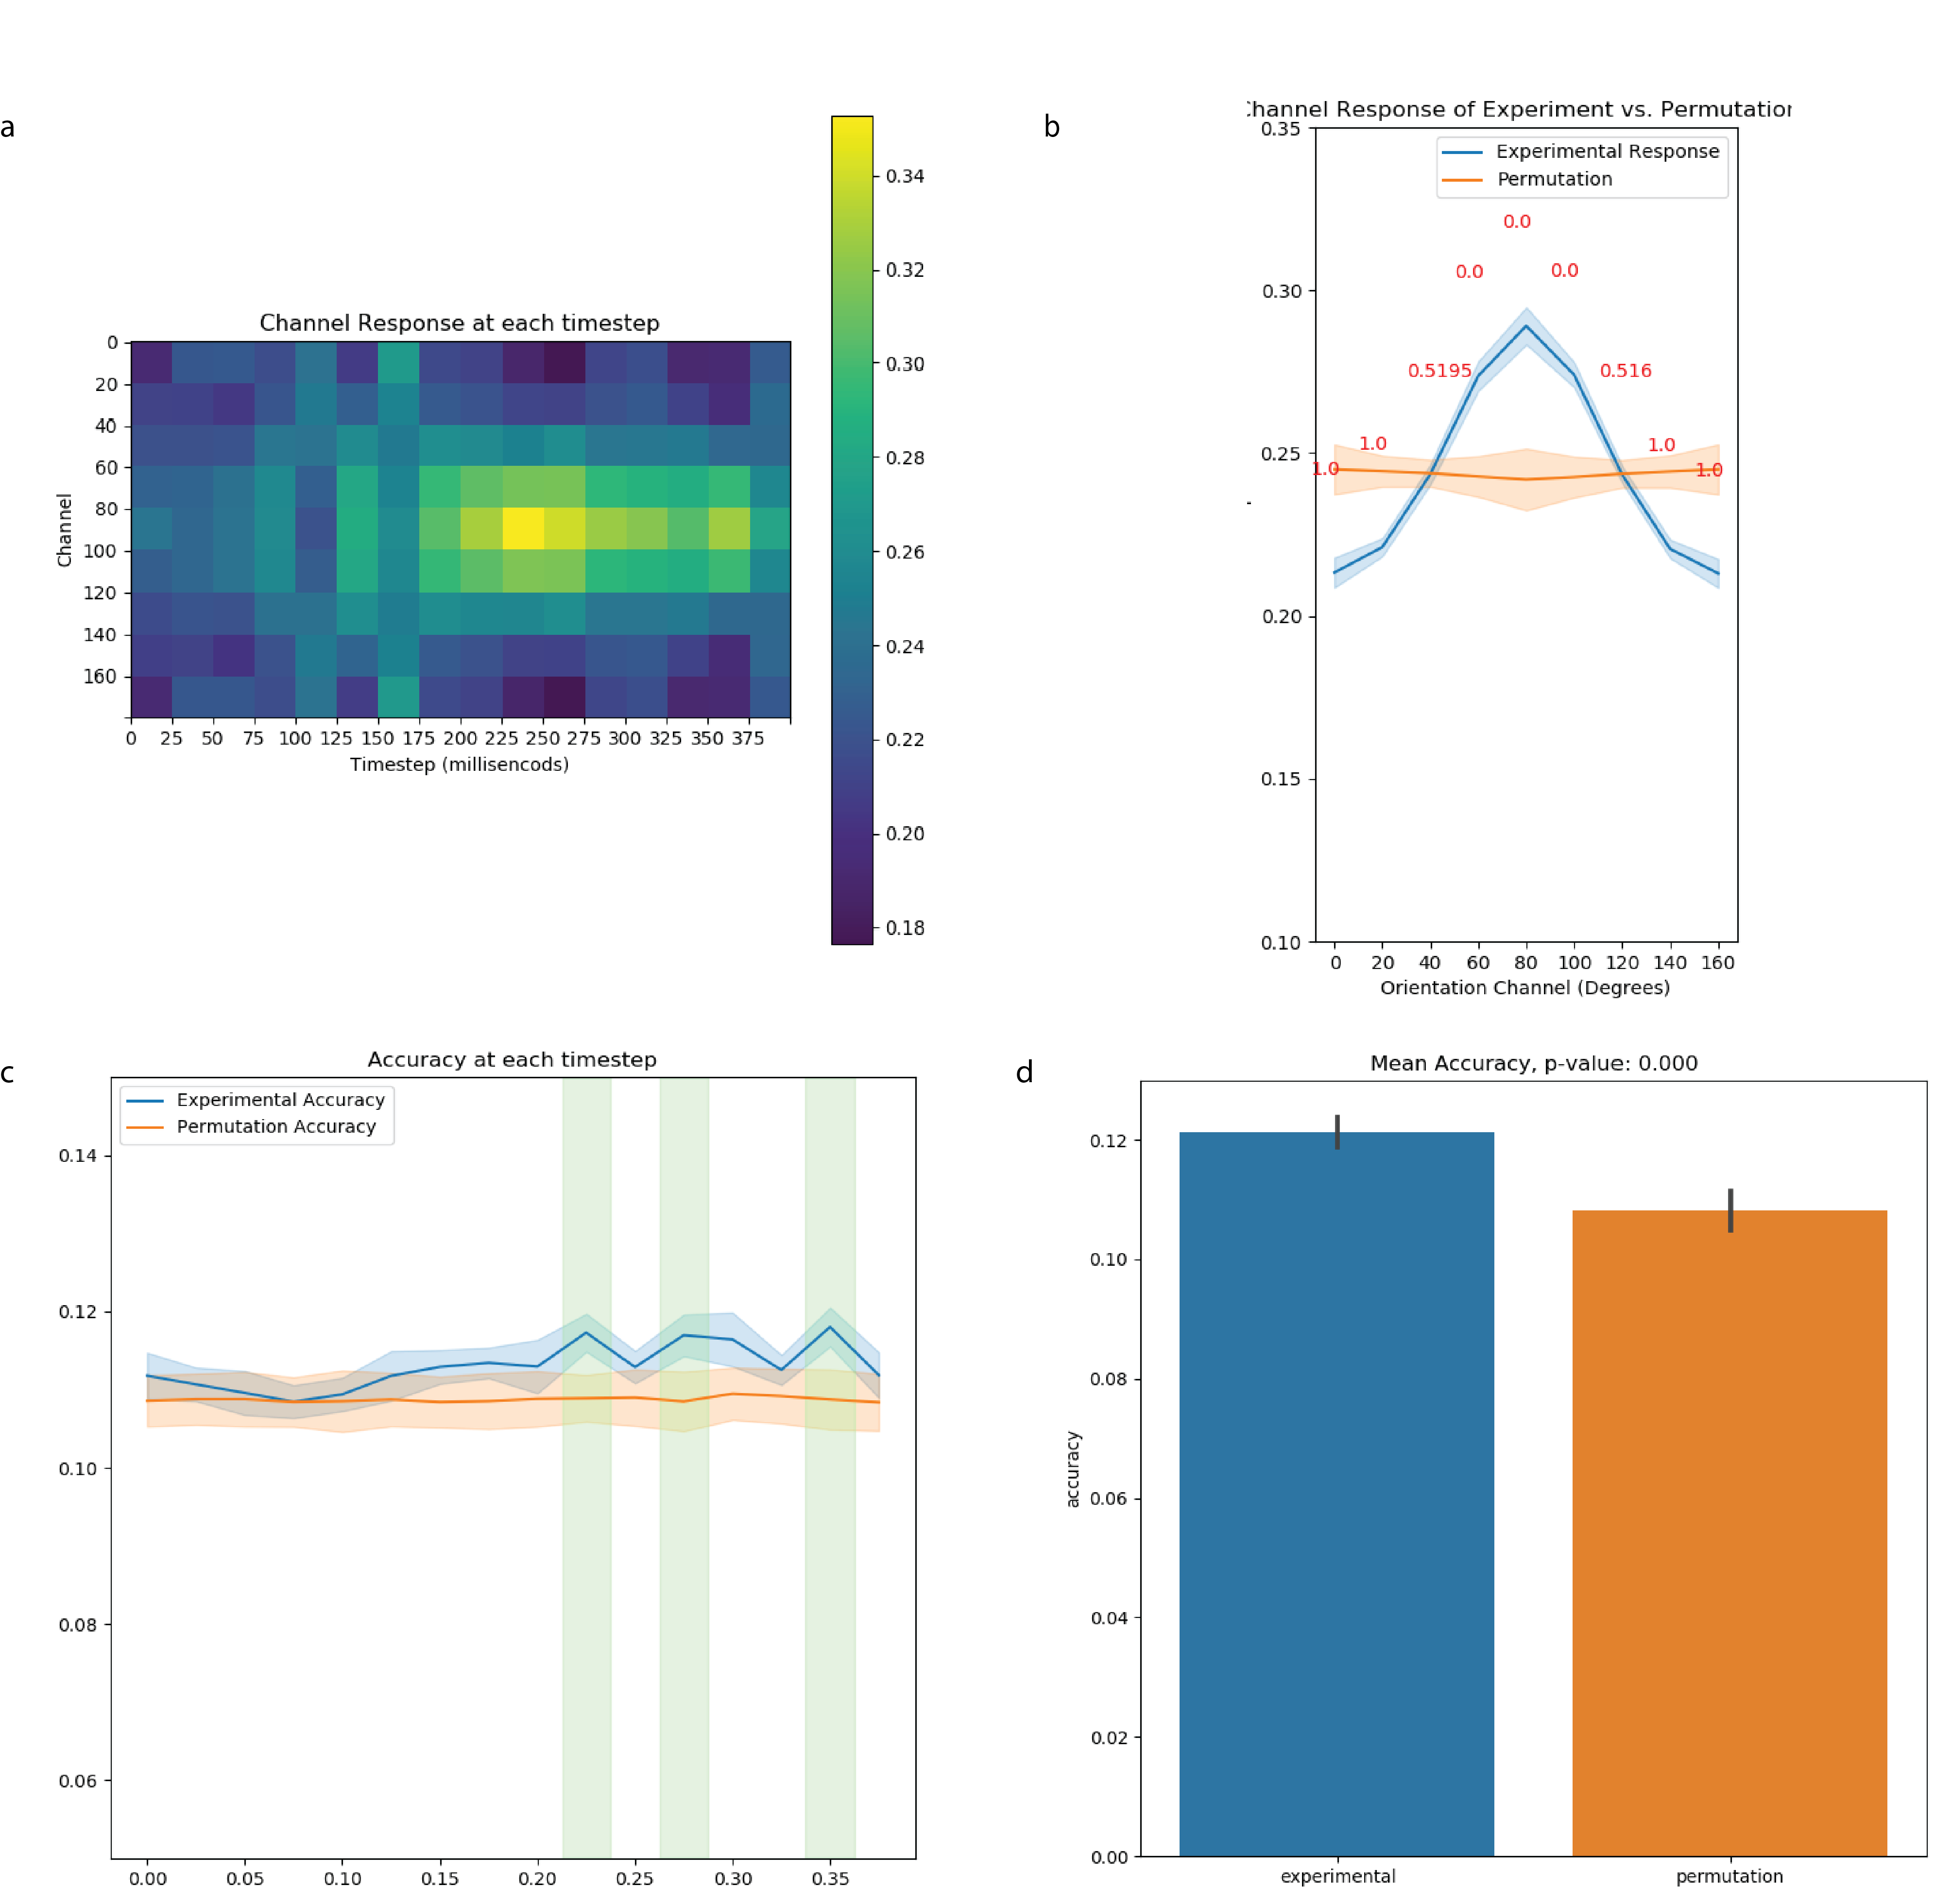
\includegraphics[scale=0.175]{figures/results/iem_results.png}
    \caption{a) IEM Channel response at 16 time steps from 0-400ms. Higher channel response values are in yellow, while lower channel response values are in blue. Channel responses begin to increase at 175ms, forming the bell curve structure found in the mean channel response. Channel responses peak at 225ms, and slowly decrease until 375ms. b) Mean channel response for the IEM compared to a permutation test. Here, there is a significant structure in the actual channel responses in comparison to the permutation test. Red numbers indicate p values for each channel. Individual trials had peaks at different orientation channels, but all channels were centered at 80 degrees for visualization. c) IEM decoding accuracy at 16 time steps. Time steps shaded green represent significant decoding time steps (p $<$ 0.05). Experimental accuracy increases beginning at 100ms after stimulus onset, and peaks around 225-350ms. d) IEM accuracy for the mean channel response. Accuracy is significantly above the permutation accuracy, with p $<$ 0.005.}
    \label{iem_results}
\end{figure}

\subsection{Serial Dependence Analysis}
\subsubsection{Behavioral performance}
Before examining serial dependence effects on decoding accuracy, we checked for a serial dependence effect in the experimental task. In Figure \ref{DoG}, we observed a significant serial dependence effect, with response orientations peaking at 1.759 degrees bias towards the previous stimulus orientation. This effect size was largest when the 1-back stimulus was 20 degrees away from the current stimulus. This effect size is consistent with previously reported serial dependence in orientation perception \citep{FRITSCHE2017590,Manassi}. These results indicate that subjects' perception of the current stimulus was pulled towards their perception of the previous target.

\begin{figure}
    \centering
    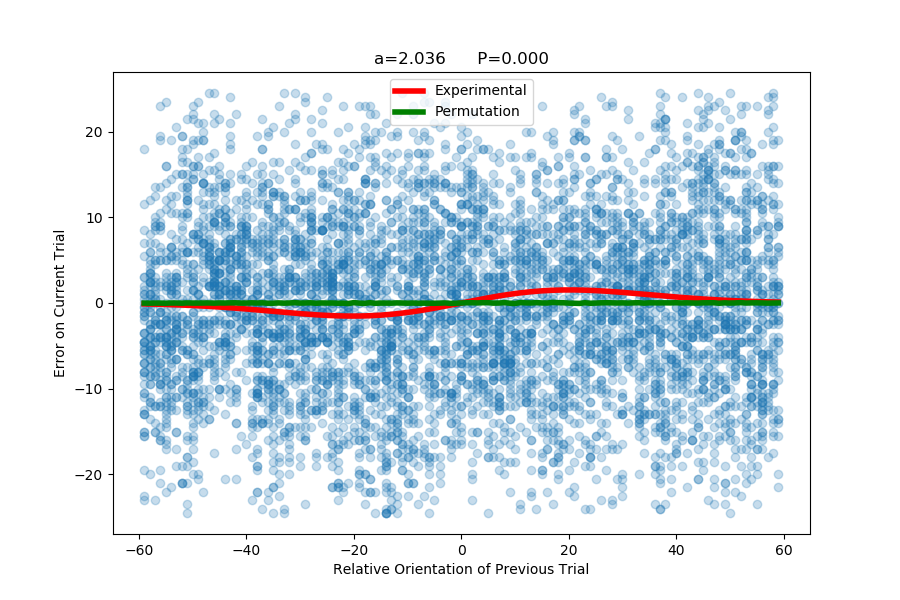
\includegraphics[scale=0.7]{figures/results/DoG_plot_v2.png}
    \caption{A comparison of relative previous orientation (previous orientation - current orientation) and error on current trial (predicted orientation - actual orientation). In red, we see a derivative of Gaussian function fit to the data points. The derivative of Gaussian had an amplitude of 1.759 degrees, achieving a p-value $<$ 0.05 according to a permutation test. In green, we see the permutation fit of the derivative of Gaussian curve, which is flat. Trials with error > 25 degrees were considered outliers and were excluded from testing. }
    \label{DoG}
\end{figure}

\subsubsection{Decoding previous orientation}
We then examined if the models from the decoding analysis had any power predicting the previous stimulus orientation from the MEG response to the current stimulus. We first investigated this previous stimulus decoding with the SVM and logistic regression, but did not find any significant results in mean accuracy or time step accuracy. This does not indicate that residual effects from the previous stimulus were not there, just that these models were unable to detect these effects. The SVM and logistic regression model already had slim accuracy improvements over a chance accuracy, so this result is expected.

However, we found very interesting results with the IEM model (Figure \ref{iem_results_prev}). Though there was no significance found in the mean channel response accuracy , there was significant decoding accuracy at 175ms (p $<$ 0.05) , and increased channel responses from 150-200ms. We also observed a bell curve structure similar to the one found in the current stimulus decoding, but it had a lower amplitude. This indicates there was some significant residual effect left by the previous stimulus, though no significant structure is revealed. Further, the peak decoding accuracy in previous stimulus decoding occurred just before current stimulus decoding accuracy became significant. This could indicate that there was a bias toward the prior stimulus shortly after the current stimulus was processed, but this bias disappeared as the current stimulus became encoded in perception.

\begin{figure}
    \centering
    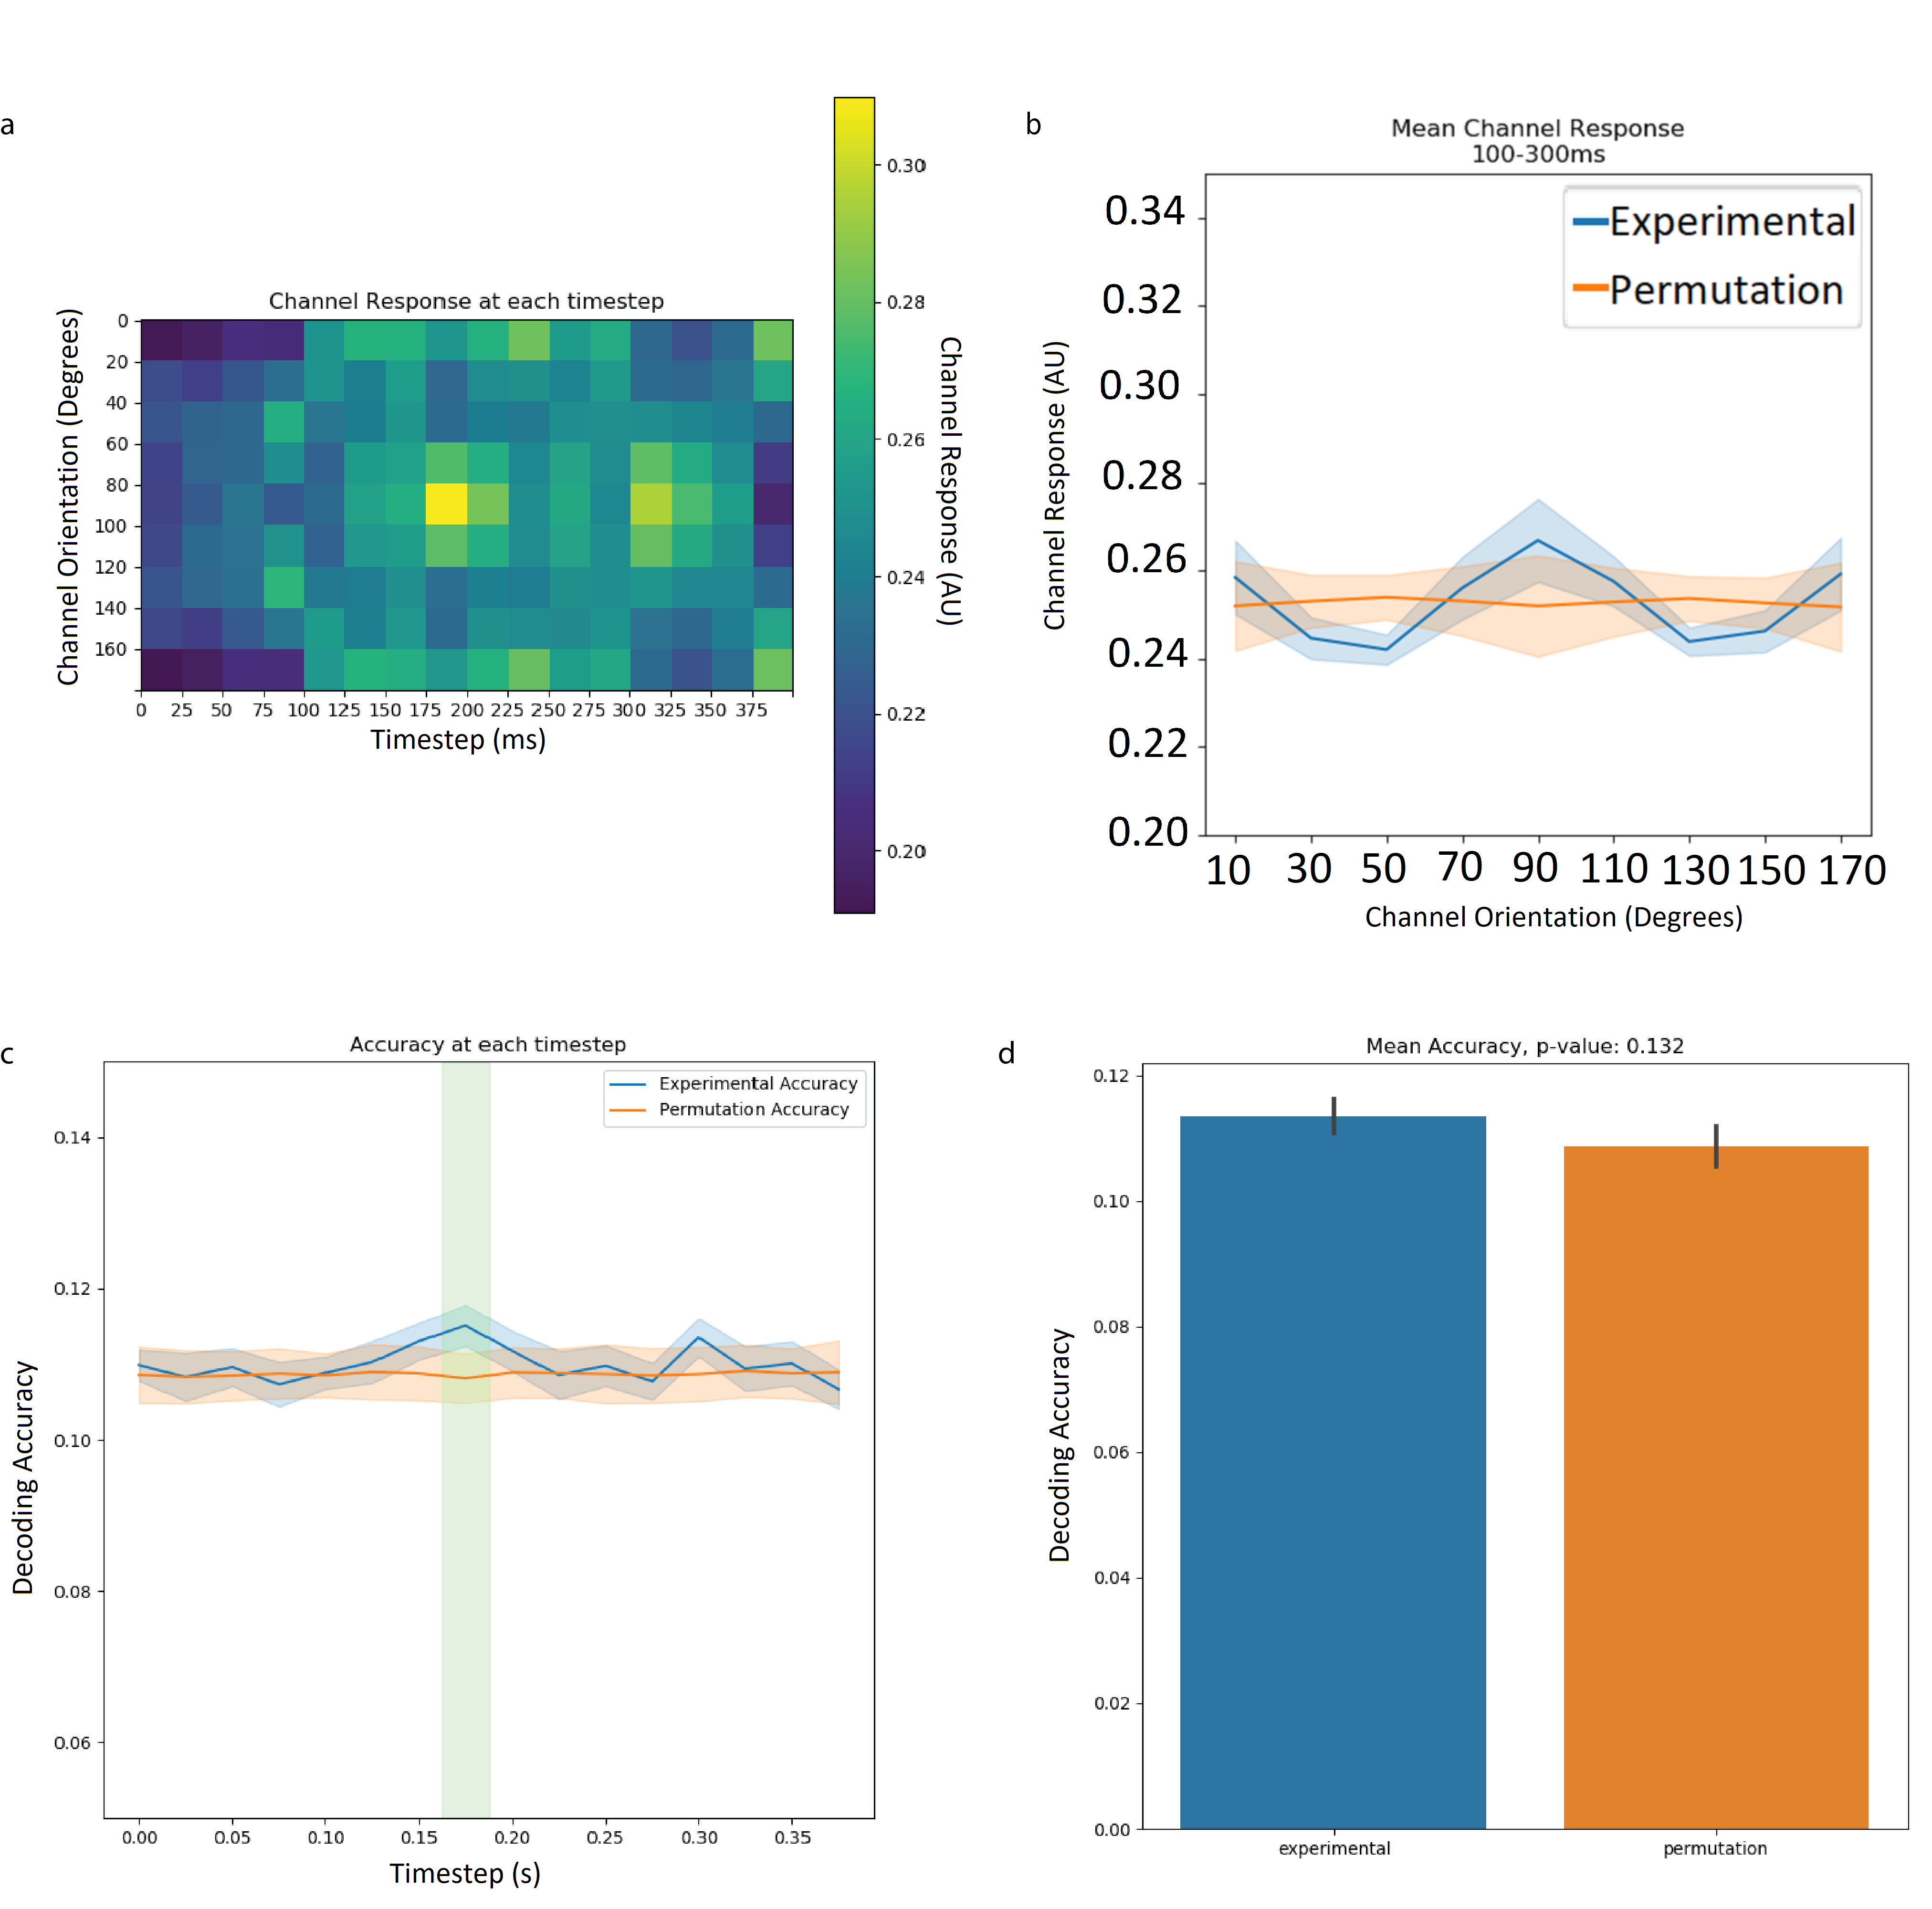
\includegraphics[scale=0.7]{figures/results/iem_results_prev.png}
    \caption{a) IEM previous decoding accuracy over 16 timesteps, averaged across 18 subjects. The accuracy at 175 ms is significant with p $<$ 0.05, (marked in green). b) IEM previous trial stimulus decoding accuracy for the mean channel response, averaged across 18 subjects. Decoding accuracy is not significant in comparison to a permutation test. c) IEM channel response for previous stimulus orientation. Higher channel responses are in yellow, lower are in blue. Channel responses peak at 175ms. Peak channel responses are lower in previous decoding (0.3 vs. 0.35). d) IEM mean channel response for previous stimulus decoding compared to a permutation test. Red values are p values for individual channel responses compared to the permutation test channel responses.}
    \label{iem_results_prev}
\end{figure}


\subsubsection{Channel response bias vs. relative previous orientation}
We finally analyzed how serial dependence might directly affect IEM decoding performance by comparing channel responses to different relative previous orientations (previous orientation - current orientation). Here, we binned channel responses according to relative previous orientation with 15 bins, centered at 0 degrees. We calculated the mean channel response for each bin, and compared each bin to randomly shuffled permutations of the bins. We repeated this for each of the 16 time steps, but did not find any bins with significant or systemic channel response bias towards or away from the previous orientation. For example, in Figure \ref{sd_all_t7}, the binned channel response at 175ms, where we had the highest previous decoding accuracy, had no significant channel responses. We are particularly interested in channel responses from -20 to +20 degrees relative previous orientation, where serial dependence effects would be strongest. There was actually channel response bias away from previous orientations in this range, but it was not significant according to this test. This lack of effect might suggest that bins were too large to gain meaningful information from, or that the orientation bins we used for decoding were too far apart to generate a meaningful serial dependence effect in decoding, considering a small serial dependence effect size.

We the performed analysis by comparing the mean of a Gaussian fit to each bin to a permutation test. There was no significance in at any time step, with P values around 0.4-0.6 for all relative previous orientation bins. At 175ms after stimulus onset, where we observed significant previous orientation decoding, there was no significance (Figure \ref{sd_all_v2_t7}).

\begin{figure}
    \centering
    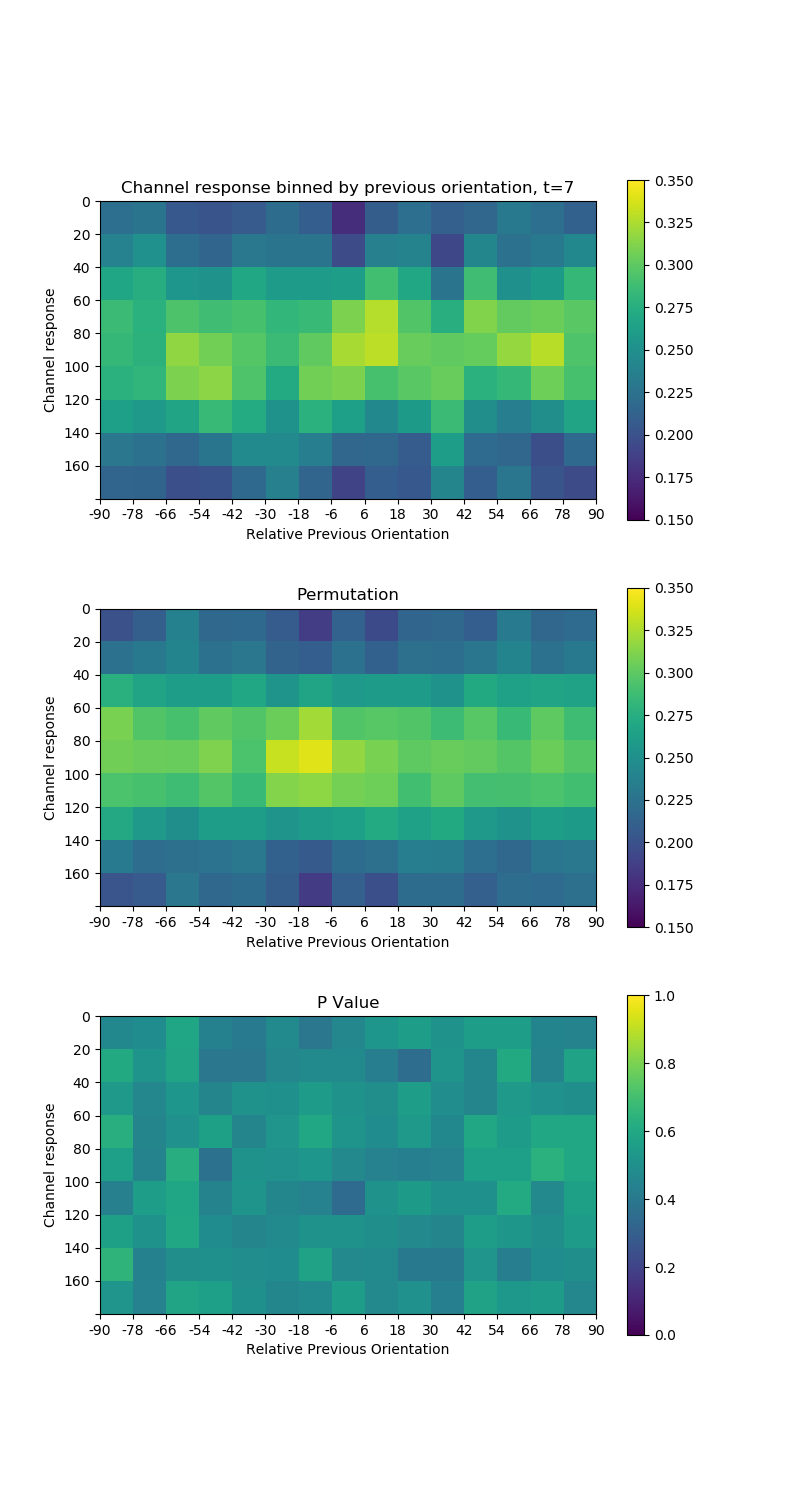
\includegraphics[scale=0.45]{figures/results/sd_all_t7.png}
    \caption{A comparison of IEM channel responses binned by relative previous orientation at 175ms. At the top, we see the binned channel responses. Blocks that are more yellow represent higher channel responses, while blue blocks have lower channel response. The middle figure shows a permutation test of the binned channels, in which bins were assigned according to shuffled relative previous orientation. The bottom figure shows the p values for each channel response block at each relative previous orientation. A low p value at a specific orientation for a bin would indicate that the block is significantly different than the average channel response for that orientation. Here, most p values hover around 0.4 to 0.6. }
    \label{sd_all_t7}
\end{figure}

\begin{figure}
    \centering
    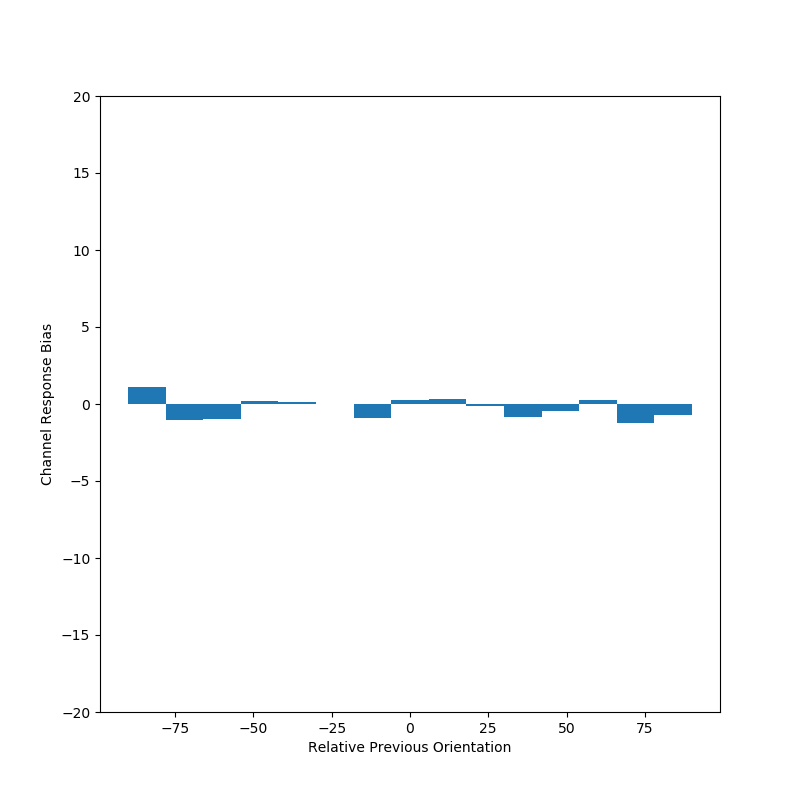
\includegraphics[scale=0.7]{figures/results/sd_all_t7_v2.png}
    \caption{Mean of Gaussian functions fit to channel responses binned by relative previous orientation at 175ms. No bin has significant deviation from 0 degrees mean in comparison to a permutation test.}
    \label{sd_all_v2_t7}
\end{figure}

\end{document}